\documentclass[border=10pt]{standalone}
\usepackage{pgfplots}
\usepgfplotslibrary{colormaps}
\pgfplotsset{compat=1.18}

\begin{document}
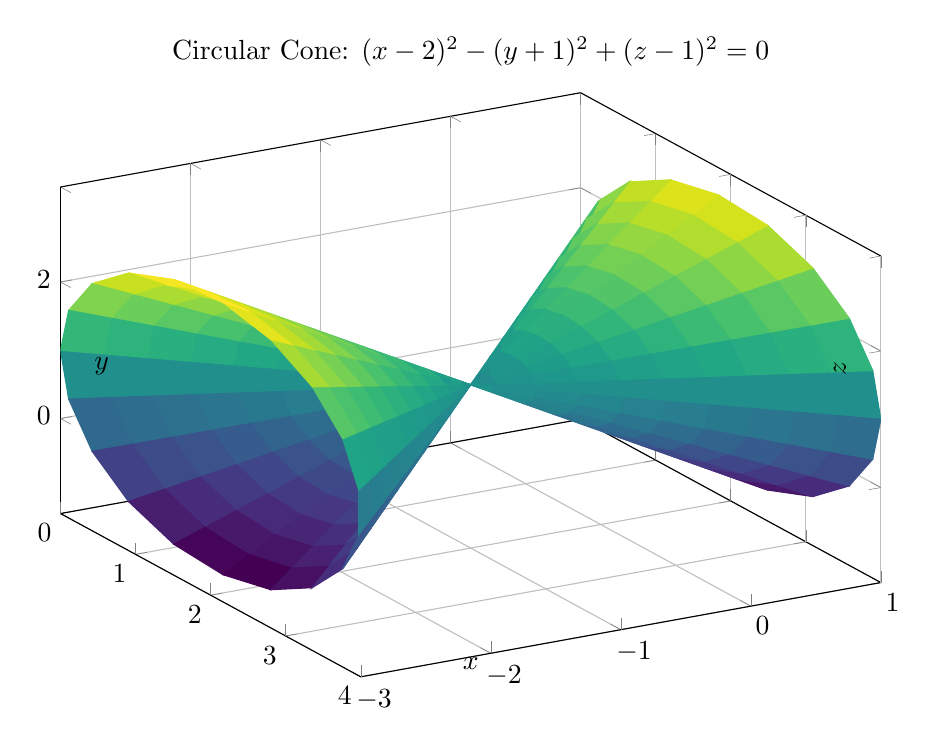
\begin{tikzpicture}
\begin{axis}[
    view={60}{30},
    xlabel={$x$},
    ylabel={$y$},
    zlabel={$z$},
    title={Circular Cone: $(x-2)^2 - (y+1)^2 + (z-1)^2 = 0$},
    colormap/viridis,
    grid=major,
    width=12cm,
    height=9cm,
    xlabel style={at={(axis description cs:0.5,0.05)}, anchor=north},
    ylabel style={at={(axis description cs:0.05,0.5)}, anchor=south},
    zlabel style={at={(axis description cs:0.95,0.5)}, anchor=west},
]
% Plot the cone surface using parametric plot
\addplot3[
    surf,
    shader=flat corner,
    samples=20,
    samples y=20,
    domain=0:360,
    y domain=-2:2,
] (
    {2 + y*cos(x)},
    {y - 1},
    {1 + y*sin(x)}
);
\end{axis}
\end{tikzpicture}
\end{document}
